

\documentclass{beamer}

\usepackage[T1]{fontenc}
\usepackage[utf8]{inputenc}
\usepackage[french,english]{babel}

\usepackage{lmodern}
\usepackage{amsthm}
\usepackage{float}
\usepackage{lmodern}%pour un meilleur rendu des polices
\usepackage{verbatim}%du texte non interprt
\usepackage{amsmath}
\usepackage{amssymb}%maths
\usepackage{xspace}
\usepackage[dvipsnames,svgnames,table]{xcolor}
\usepackage{listings}
\usepackage{fancyhdr}
\usepackage{etoolbox}
\usepackage{titlesec}
\usepackage{titletoc}
\usepackage{lastpage}
\usepackage{hyperref}
\usepackage{ctable} % for \specialrule command
\usepackage{cite}
\usepackage{algorithm2e}
\usepackage{alltt}
\usepackage{array}
\usepackage{mdwmath}
\usepackage{mdwtab}
\usepackage{eqparbox}
\usepackage{subfig}
\usepackage{dblfloatfix}
\usepackage{url}
\usepackage{tipa}
\usepackage{stmaryrd}
\usepackage{upgreek}
\usepackage{mathrsfs}
\usepackage{ulem}
\usepackage{cancel}

\graphicspath{{img/}}
\DeclareGraphicsExtensions{.pdf,.jpeg,.jpg,.png}


\newcommand{\ccite}[1]{\textbf{\cite{#1}}}
\newcommand{\pd}[2]{\dfrac{\partial #1}{\partial #2}}
\newcommand{\od}[2]{\dfrac{\mathscr{D}_a #1}{\mathscr{D} #2}}
\newcommand{\tensor}[1]{\mathbf{#1}}
\renewcommand{\vector}[1]{\overrightarrow{#1}}

\newcommand{\Tau}{\tensor{\mathlarger{\uptau}}}
\renewcommand{\v}{\vector{u}}
\newcommand{\W}{\tensor{W\left( \v \right)}}
\newcommand{\D}{\tensor{D\left( \v \right)}}
\newcommand{\grad}{\vector{\nabla}}
\newcommand{\gradv}{\tensor{\nabla\v}}
\renewcommand{\div}[1]{div \left( #1 \right)}
\newcommand{\divv}[1]{\vector{div} \left( #1 \right)}
\newcommand{\UU}{\mathcal{U}}
\newcommand{\VV}{\mathcal{U}}
\newcommand{\M}{\mathcal{M}}
\newcommand{\A}[2]{\mathcal{A}_{#1}\left( #2 \right)}
\newcommand{\Uu}{\UU^{n}}
\newcommand{\Uv}{\UU^{n+\theta}}
\newcommand{\Uw}{\UU^{n+1-\theta}}
\newcommand{\Ux}{\UU^{n+1}}
\newcommand{\Uk}{\UU^{k}}
\newcommand{\Ukk}{\UU^{k+1}}
\newcommand{\Vk}{\VV^{k}}
\newcommand{\Vkk}{\VV^{k+1}}
\newcommand{\Tauk}{\Tau^{k+1}}
\newcommand{\vk}{\v^{k+1}}
\newcommand{\pk}{p^{k+1}}
\newcommand{\Dk}{\tensor{D\left( \vk \right)}}

\definecolor{lightgray}{gray}{0.9}
\definecolor{titlecolor}{RGB}{0,0,200}
\definecolor{subtitlecolor}{RGB}{0,0,153}
\definecolor{textcolor}{RGB}{0,128,255}
\definecolor{RoyalPurple}{RGB}{102,51,153}
\definecolor{ForestGreen}{RGB}{34,139,34}


\newcommand{\colbox}[1]{\colorbox{lightgray}{$ #1 $}}

\newcommand{\stitle}[2][0.3cm] { 
    {\normalsize \textcolor{titlecolor}{\textbf{#2}}} 
    \vspace{#1} 
}

\newcommand{\ssubtitle}[1]{ {\footnotesize \textcolor{subtitlecolor}{\textbf{#1}}} }

\newcommand{\stress}[1]{\textcolor{textcolor}{#1}}

\newcommand{\hidecontent}[2][0.25]{{% \hidecontent[<transparency>]{<stuff>}
  \setbox9=\hbox{#2}% Store <stuff> in \box9 to obtain height/width
  \transparent{#1}\ooalign{\usebox9\cr\color{white}\rule{\wd9}{\ht9}\cr}}}



\usetheme{Frankfurt}
\def\beamertemplatetransparentcoveredmedium{\setbeamercovered{transparent=40}}
\def\beamertemplatetransparentcoveredhard{\setbeamercovered{transparent=20}}
\beamertemplatetransparentcoveredmedium
\setbeamertemplate{bibliography item}[triangle]
\addtobeamertemplate{footline}{\hfill\insertframenumber/\inserttotalframenumber\hspace{2em}\null}

\begin{document}


\title{\Large Scattered Data Interpolation using Wavelet Trees}
\author[Keck]{\Large Jean-Baptiste Keck}
\institute[MSIAM]{\Large \bsc{M2 Msiam}}
\date{\large Paper Review\\ 10/02/2015}


\begin{frame}
    \titlepage
\end{frame}


\begin{frame}{Interpolating wavelets} 

    \titleframe{Interpolating wavelets}

    \only<2->{

        \stitle{Building interpolation wavelets}
        \footnotesize

        \uncover<2->{
            \begin{itemize}
                \item Classical interpolation tools can be fitted into a MRA framework.
            \end{itemize}
        }

        \uncover<3->{
            \begin{block}{Interpolating scaling function}
                $\P$ is an interpolating scaling function 
                $
                \Leftrightarrow
                \left\{
                    \begin{array}{l c l l}
                        \P(0) & = & 1 & \\
                        \P(k) & = & 0 & \forall\ k \in \Z^* \\
                    \end{array}
                    $
                \end{block}
            }

            \begin{itemize}
                \item<4-> Built as infinite convolution of discrete filters
                    $\Ph(\nu) = \prod_{k=1}^{+\infty} m_0(\frac{\nu}{2\pi})$ 
                    \vskip 0.3cm
                \item<5-> Interpolating property can be expressed as $m_0(\nu) + m_0(\nu + \pi) = 1$
                    \vskip 0.3cm
                \item<6-> $\P$ has compact support $\Leftrightarrow h_n$ is finite $\Rightarrow$ Approximation order is finite 
                    \vskip 0.3cm
                \item<7-> \textbf{Families :} Splines functions, \alert{Deslauriers-Dubuc interpolating wavelets}
            \end{itemize}
        }
    \end{frame}

    \begin{frame}{Deslauriers-Dubuc interpolating wavelets} 
        \setbeamercovered{invisible}
        \ssubtitle{Lagrange interpolation :}
        \footnotesize

        \begin{itemize}
            \item Can explicitely compute filter coefficients \alert{$h_n$} with Lagrange polynomials of order $\alert{p}\ \forall n \in \llbracket -2p+1, 2p-1 \rrbracket$.
        \end{itemize}

        \vskip 0.2cm

        \uncover<2->{
            \ssubtitle{Dyadic refinement scheme :}
            \vskip -0.3cm
            \begin{figure}[H]
                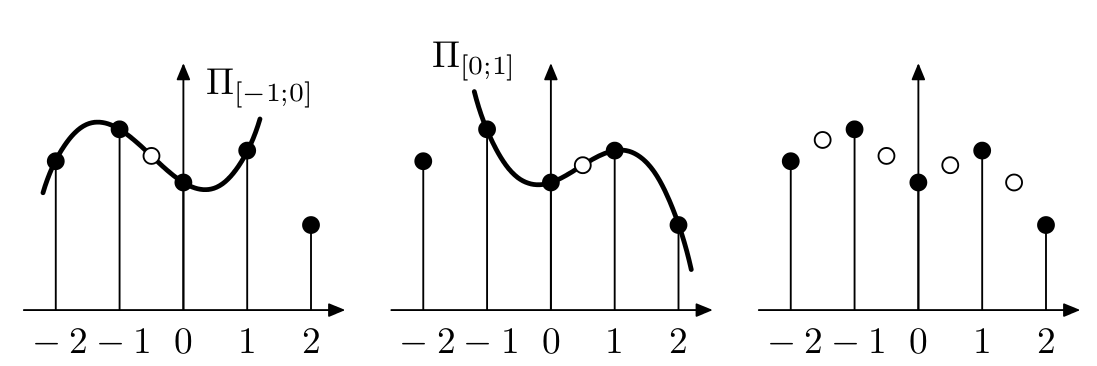
\includegraphics[scale=0.2]{lagrange}
            \end{figure}
        }

        \uncover<3->{
            \begin{block}{Low pass filter coefficients $h_n$}
                $
                \begin{array}{l cc c cc r}
                    m_0[0] = 1 && 
                    m_0[2k] = 0 \textrm { if } k \in \Z^* &&
                    m_0[k] = 0 \textrm{ if } |k| \geq 2p& \\
                    \\
                    \multicolumn{7}{l}{
                        m_0[\pm (2k-1)] = \dfrac{(-1)^{k+1}(2p)!^2}{2^{4p}p!^2(p-k)!(p+k-1)!(2k-1)}\ \ \ \forall k \leq p
                    }
                \end{array}
                $
            }
        \end{block}
    \end{frame}

    \begin{frame}{Generation of the coefficients} 
        \ssubtitle{Just evaluate Lagrange polynomials to get the $h_n$ :}
        \begin{figure}[H]
            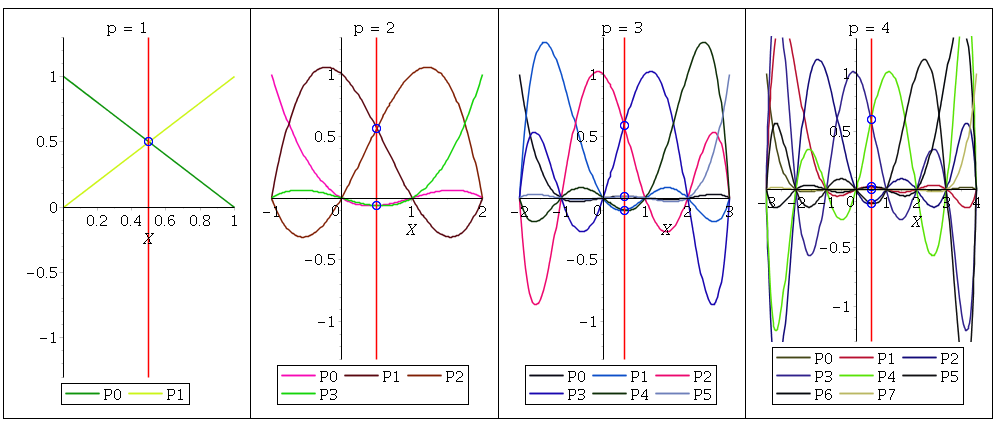
\includegraphics[scale=0.33]{coefficients}
        \end{figure}
    \end{frame}

    \begin{frame}{Generation of the scaling function} 

        \footnotesize

        \ssubtitle{Generate $\P_p$ at resolution $2^{-j}$ with j convolutions $\delta_{x,0} \ast h_n^p \ast \cdots \ast h_n^p$ :}

        \only<1>{
            \begin{figure}[H]
                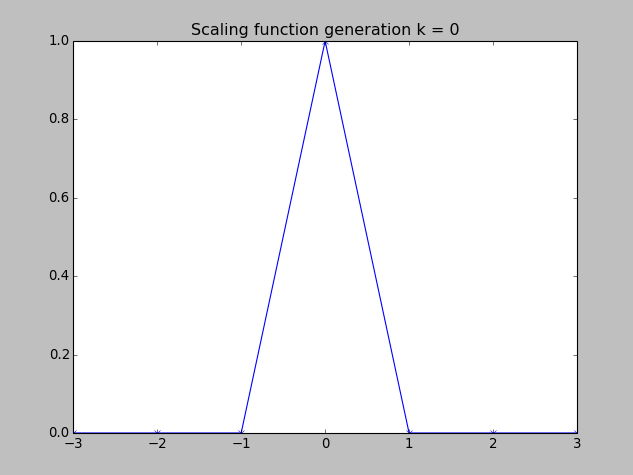
\includegraphics[scale=0.4]{scaling_10}
            \end{figure}
        }
        \only<2>{
            \begin{figure}[H]
                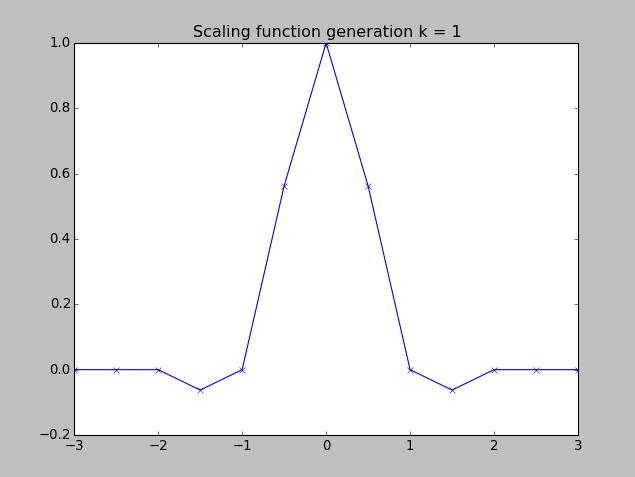
\includegraphics[scale=0.4]{scaling_11}
            \end{figure}
        }
        \only<3>{
            \begin{figure}[H]
                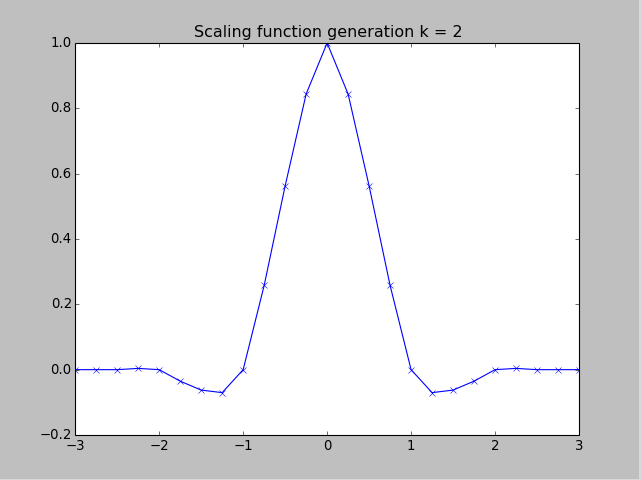
\includegraphics[scale=0.4]{scaling_12}
            \end{figure}
        }
        \only<4>{
            \begin{figure}[H]
                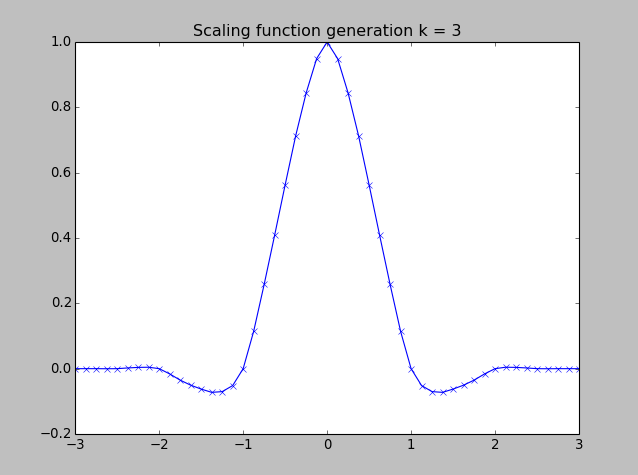
\includegraphics[scale=0.4]{scaling_13}
            \end{figure}
        }
        \only<5>{
            \begin{figure}[H]
                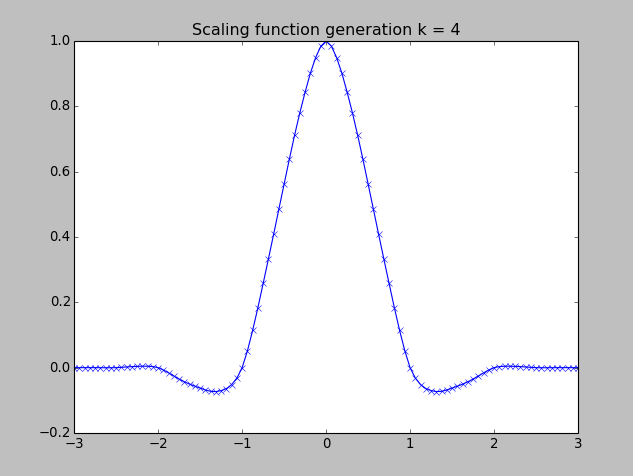
\includegraphics[scale=0.4]{scaling_14}
            \end{figure}
        }
        \only<6>{
            \begin{figure}[H]
                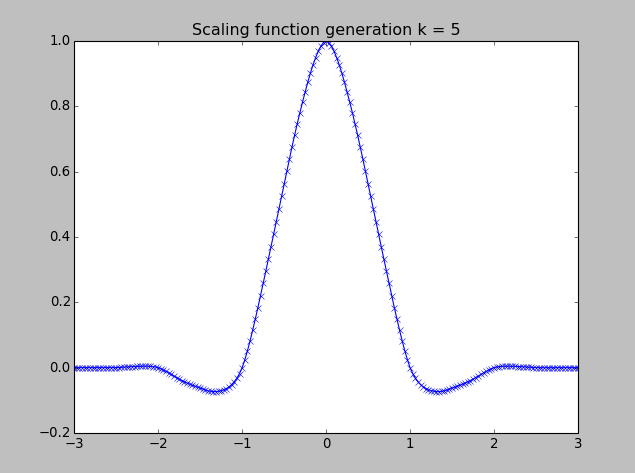
\includegraphics[scale=0.4]{scaling_15}
            \end{figure}
        }
        \only<7>{
            \begin{figure}[H]
                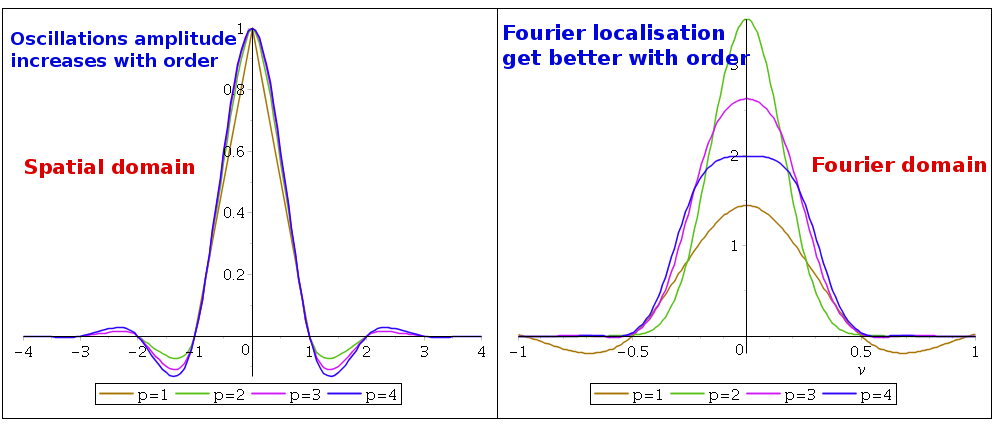
\includegraphics[scale=0.32]{dd_scaling}
            \end{figure}
        }
    \end{frame}


    \begin{frame}{Properties} 

        \ssubtitle{Basis definition in the dyadic case:}
        \begin{itemize}
            \item<1->  Scaling function : $\P$(x) is of order p
            \item<2->  Mother wavelet : $\Psi(x) = \P(2x - 1)$
            \item<3->  Wavelet family : $\Psi_{jk} = \Psi(2^j x - k)$
            \item<4->  Basis : $\mathcal{B}_0 = \{ \Psi_{jk}\ |\ \underbrace{j = 0}_{V_0} \textrm{ \alert{or} } \underbrace{(j,k) \in \N^* \times (2\Z + 1)}_{W_{j-1}} \}$
        \end{itemize}

        \ssubtitle{Properties :}

        \begin{itemize}
            \item<5-> Symmetry
            \item<6-> Finite support $\subset [-2p+\frac{1}{2}, 2p-\frac{1}{2} ]$
            \item<7-> \alert{No orthogonality} $\Rightarrow$ need to solve a linear system
            \item<8-> $2p$ vanishing moments
        \end{itemize}

        \ssubtitle{Wavelets on the interval (boundary problems) :}
        \begin{itemize}
            \item<9-> Take \alert{boundary filters of lower order}
        \end{itemize}

    \end{frame}

    \begin{frame}{Wavelets on the interval : case $\Omega = [0,1]$ } 

        \ssubtitle{Boundary filters : Lowest resolution => Highest resolution}

        \only<1>{
            \begin{center}
                $V_0$
            \end{center}
            \vskip -0.3cm
            \begin{figure}[H]
                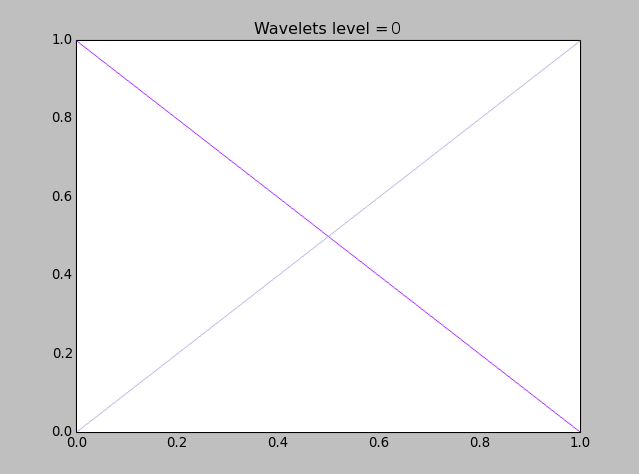
\includegraphics[scale=0.4]{interval_0}
            \end{figure}
        }
        \only<2>{
            \begin{center}
                $W_0$
            \end{center}
            \vskip -0.3cm
            \begin{figure}[H]
                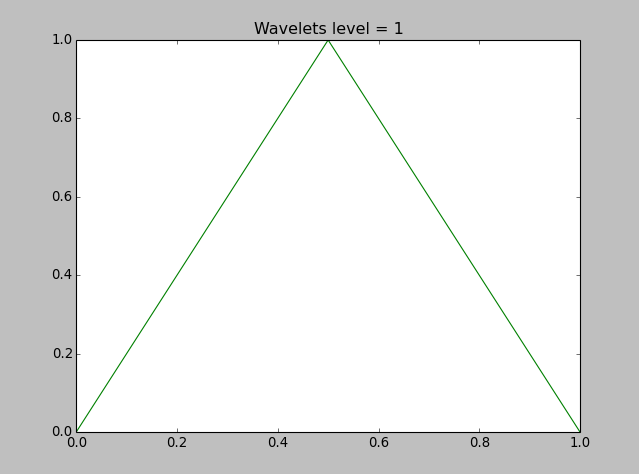
\includegraphics[scale=0.4]{interval_1}
            \end{figure}
        }
        \only<3>{
            \begin{center}
                $W_1$
            \end{center}
            \vskip -0.3cm
            \begin{figure}[H]
                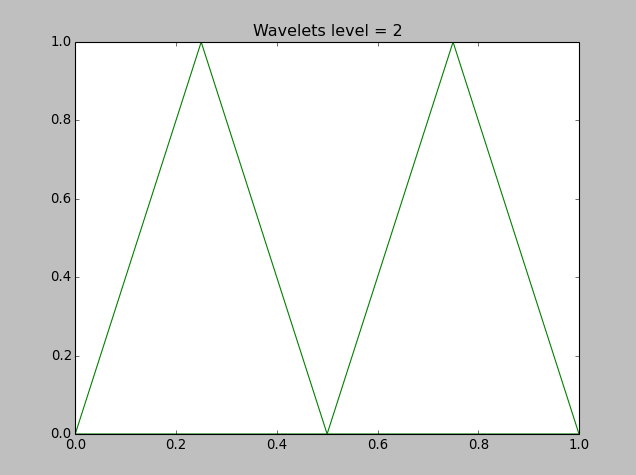
\includegraphics[scale=0.4]{interval_2}
            \end{figure}
        }
        \only<4>{
            \begin{center}
                $W_2$
            \end{center}
            \vskip -0.3cm
            \begin{figure}[H]
                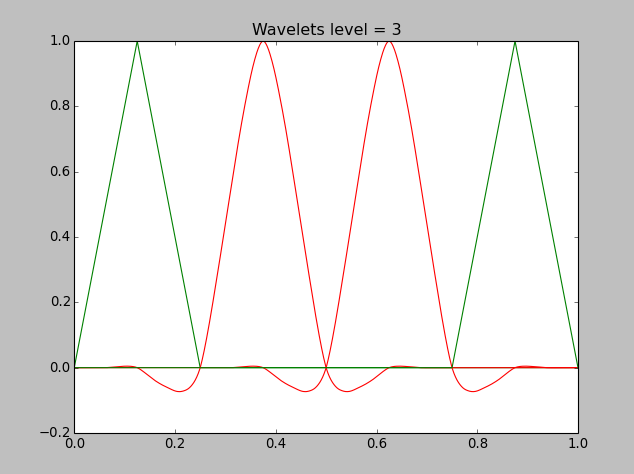
\includegraphics[scale=0.4]{interval_3}
            \end{figure}
        }
        \only<5>{
            \begin{center}
                $W_3$
            \end{center}
            \vskip -0.3cm
            \begin{figure}[H]
                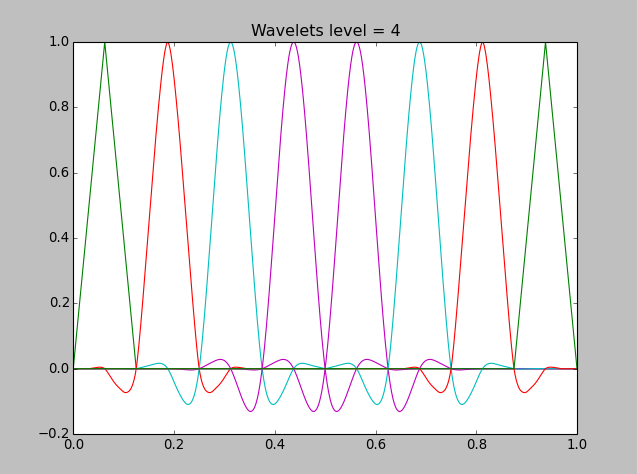
\includegraphics[scale=0.4]{interval_4}
            \end{figure}
        }
        \only<6>{
            \begin{center}
                $W_4$
            \end{center}
            \vskip -0.3cm
            \begin{figure}[H]
                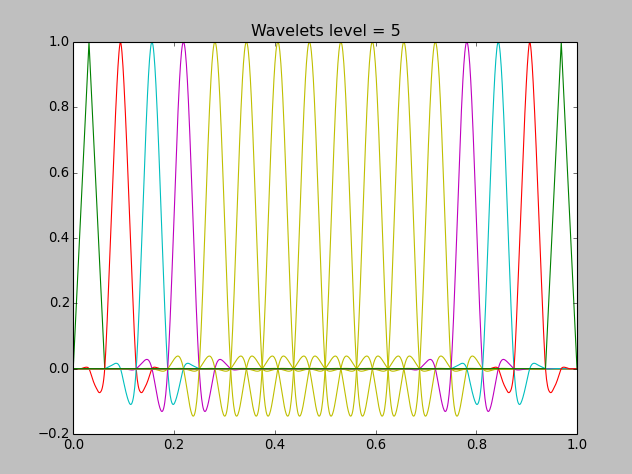
\includegraphics[scale=0.4]{interval_5}
            \end{figure}
        }

    \end{frame}


    \begin{frame}{Approximation in wavelet bases} 

        \titleframe{Wavelet tree approximation}

        \only<2->{

            \stitle{Different approximations possible in wavelet bases :}
            \footnotesize

            \begin{itemize}

                    \uncover<2->{
                    \item \textbf{Exact wavelet decomposition :}
                        {\scriptsize 
                            $f = 
                            \displaystyle \sum_{j=0}^{\infty} \displaystyle \sum_{k\in\Z} \langle f \mid \Psi_{jk} \rangle \Psi_{jk}
                        = \displaystyle \sum_{j=0}^{\infty} \displaystyle \sum_{k\in\Z} \alert{d_{jk}} \Psi_{jk}$}
                    }

                    \uncover<3->{
                    \item \textbf{Linear approximation $\A_{lin}^{\alpha}$:} 
                        $f \simeq \displaystyle \sum_{j=0}^{\alert{J}} \displaystyle \sum_{k\in\Z} d_{jk} \Psi_{jk}$

                        \vskip 0.3cm
                    }
                    \uncover<4->{
                    \item \textbf{Non-linear approximation} $\A^{\alpha}$ (best N-terms approximation) : 
                        $
                        \abs{d_{j_0,k_0}} \geq
                        \abs{d_{j_1,k_1}} \geq
                        \cdots \geq
                        \abs{d_{j_{N-1},k_{N-1}}}
                        \Rightarrow
                        f \simeq \displaystyle \sum_{i=0}^{\alert{N}} 
                        d_{j_i,k_i}
                        \ \psi_{j_i,k_i}
                        $

                        \vskip 0.1cm
                    }
                    \uncover<5->{
                    \item \stress{\textbf{Tree approximation}} $\T^{\alpha}$ :  Build a wavelet tree with following relationship
                        \vskip 0.1cm
                        \begin{center}
                            $
                            (j,k)\ \R\ (j',k') 
                            \Leftrightarrow
                            \left\{
                                \begin{array}{l c l}
                                    j' & = & j + 1 \\
                                    k' & \in & \{2k - 1, 2k + 1\} \\
                                \end{array}
                                $
                            \end{center} 

                            \alert{Tree approximation spaces are close to non-linear spaces} (because singularities are located).
                        }
                \end{itemize}
            }

        \end{frame}

        \begin{frame}{Example of wavelet tree structure} 
            \begin{figure}[H]
                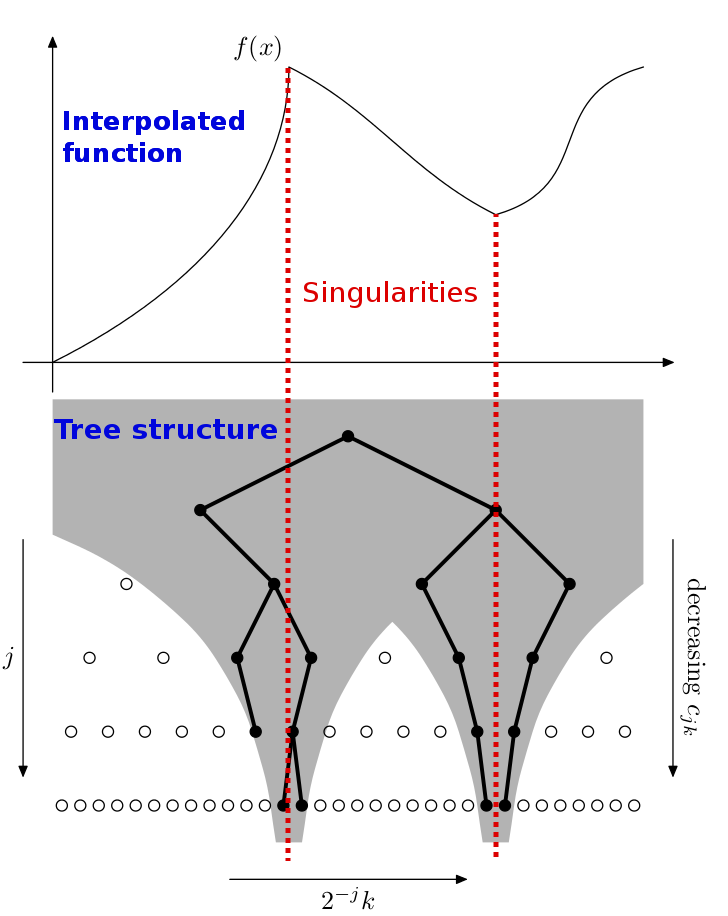
\includegraphics[scale=0.23]{tree_example}
            \end{figure}
        \end{frame}

        \begin{frame}{Scattered data interpolation}

            \titleframe{Scattered data interpolation using wavelet trees}
            \only<2->{

                \stitle{Scattered data interpolation with wavelet trees:}
                \footnotesize
                \begin{itemize}
                    \item<2-> \textbf{Input:} Set of \alert{N samples $\X \subset \mathbb{R}$} with corresponding sample values $\alert{f_{\X}} = \{ f(x) \ | \ x \in \X \}$
                    \item<3-> \stress{Samples are not aligned with wavelet centers $2^{-j}k$}
                    \item<4-> \textbf{Output:} $\alert{\J_S} \subset (0,\mathbb{Z}) \cup \mathbb{N^*} \times (2\mathbb{Z}+1)$ and coefficients \alert{$c_{jk}$} st.

                        \vskip 0.2cm

                        \uncover<4->{
                            $
                            \left\{
                                \begin{array}{l} 
                                    \forall\ (j',k') \in \mathbb{N^*}\times (2\mathbb{Z}+1) 
                                    \ \ \ \exists\ (j,k) \in \J_S\ \ \ \ (j,k)\ \R\ (j',k') \\
                                    f \simeq \displaystyle \sum_{(j,k) \in \J_S} c_{jk} \Psi_{jk}\\
                                \end{array}
                                $
                            }
                    \end{itemize}

                    \vskip 0.3cm
                    \stitle{Three step tree interpolation method:}
                    \begin{itemize}
                        \item<5-> \stress{\textbf{Allocation :}} Build one-one mapping from $\X$ to wavelet basis $\B_{\J}$
                        \item<6-> \stress{\textbf{Subsystem selection :}} Remove bad samples with a geometric criterion, new wavelet basis is $B_{\J_S} \subset \B_{\J}$
                        \item<7-> \stress{\textbf{System solving:}} Solve a linear system to find $c_{ij}\ \forall (i,j) \in \J_S$
                    \end{itemize}
                }

            \end{frame}

            \begin{frame}{Example function}
                $\mathbf{f(x) = cos(75x)\ e^x\ cos(10x)}$ on \alert{$\Omega = [0,1]$} approximated at order \alert{$p = 10$} with up to \alert{$N = 100$} uniformly distributed samples :

                \only<1>{
                    \begin{figure}[H]
                        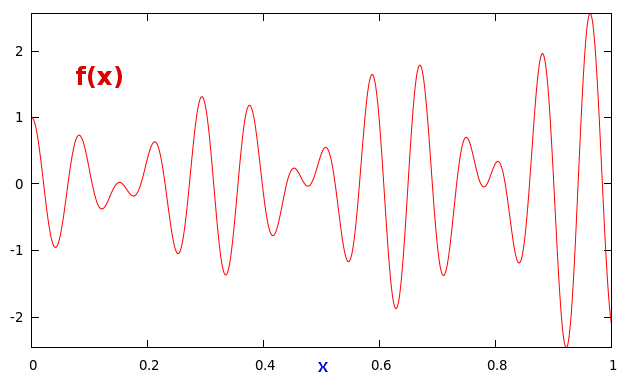
\includegraphics[scale=0.4]{f}
                    \end{figure}
                }
                \only<2>{
                    \begin{figure}[H]
                        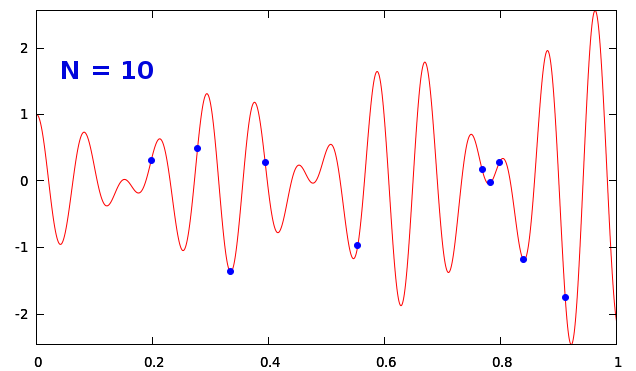
\includegraphics[scale=0.4]{f_10}
                    \end{figure}
                }
                \only<3>{
                    \begin{figure}[H]
                        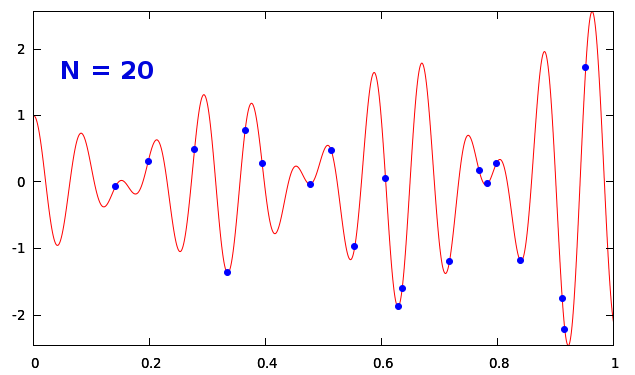
\includegraphics[scale=0.4]{f_20}
                    \end{figure}
                }
                \only<4>{
                    \begin{figure}[H]
                        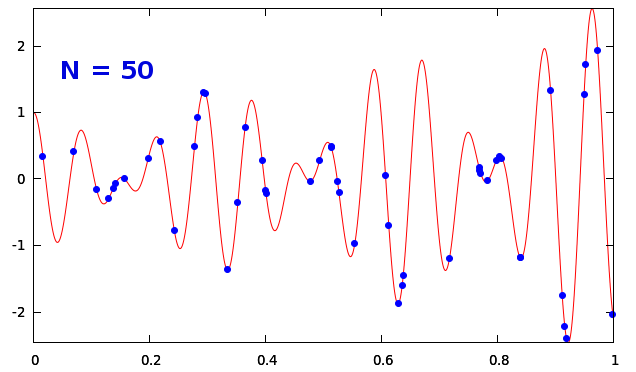
\includegraphics[scale=0.4]{f_50}
                    \end{figure}
                }
                \only<5>{
                    \begin{figure}[H]
                        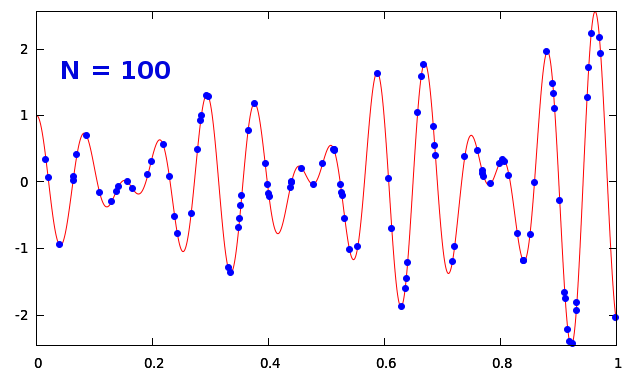
\includegraphics[scale=0.4]{f_100}
                    \end{figure}
                }

            \end{frame}

            \begin{frame}{First step : Allocation}
                \stitle{Allocation :}
                \footnotesize

                The goal is to \stress{select a wavelet subfamily} to build an interpolating basis $\stress{\B_\J} \subset \B_0$.

                \begin{itemize}
                    \item<2-> Build a subfamily which provides a function that is a priori smooth
                        \uncover<2->{
                            $\Rightarrow$ \alert{Low resolution wavelets should be preferred}.
                        }
                    \item<3-> Select high resolution wavelets \alert{only where the density of measures is high}.
                \end{itemize}

                \uncover<4->{
                    \begin{block}{Admissible allocation}
                        $\A : \X \to \J_\A \subset (0,\Z) \cup \N^* \times (2\Z+1)$ is an admissible allocation
                        $\Leftrightarrow$
                        \vskip 0.3cm 
                        $
                        \left\{
                            \begin{array}{l}
                                \forall\ x_i \in \X,\ \A(x_i) = (j,k)\ 
                                \Rightarrow \ x \in B_{jk} (\textrm{\alert{attraction basin} of the wavelet } \Psi_{jk} ) \\
                                \A(x) = (j,k), x \in B_{j'k'} \textrm{ with } j' < j 
                                \Rightarrow \exists x' \in \X \textrm{ such that } \A(x') = (j',k')
                            \end{array}
                            \right.
                            $
                        \end{block}
                    }
                \end{frame}


                \begin{frame}{First step : Allocation}
                    \begin{block}{Order on the allocations}
                        \footnotesize
                        $\A \geq \A' \Leftrightarrow \exists j_0 \in \N \textrm{ such that }$
                        \vskip 0.1cm
                        $

                        \left\{
                            \begin{array}{l}
                                \textrm{Allocations are the same up to level } $\ j_0$ \\
                                \forall k \in \Z 
                                \ \ (j_0, k) \in \J_\A \Rightarrow 
                                \abs{\A^{-1}(j_0,k) - \nu_{j_0,k}}
                                \leq
                                \abs{\A'^{-1}(j_0,k) - \nu_{j_0,k}}
                            \end{array}
                            \right.
                            $
                        \end{block}

                        \uncover<2->{
                            \begin{block}{Theorem}
                                Let $\X$ be a set of measure points. Then at least one of the following sentence is true:
                                \begin{itemize}
                                    \item $\exists$! optimal allocation $\A$
                                    \item $\exists$ two equivalent allocations $\A \sim \A'$
                                \end{itemize}
                            \end{block}
                        }

                    \end{frame}

                    \begin{frame}{Example of allocation}
                        \only<1>{
                            \begin{figure}[H]
                                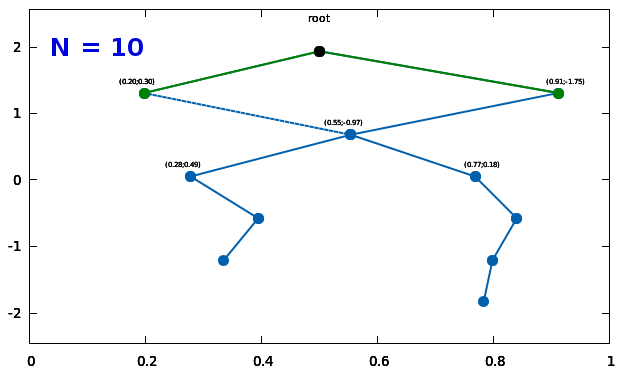
\includegraphics[scale=0.5]{tree_10}
                            \end{figure}
                        }
                        \only<2>{
                            \begin{figure}[H]
                                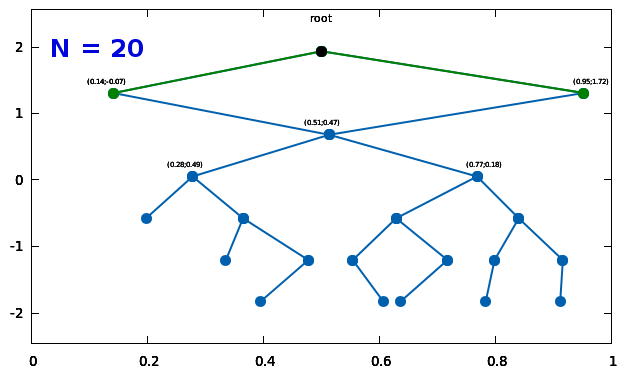
\includegraphics[scale=0.5]{tree_20}
                            \end{figure}
                        }
                        \only<3>{
                            \begin{figure}[H]
                                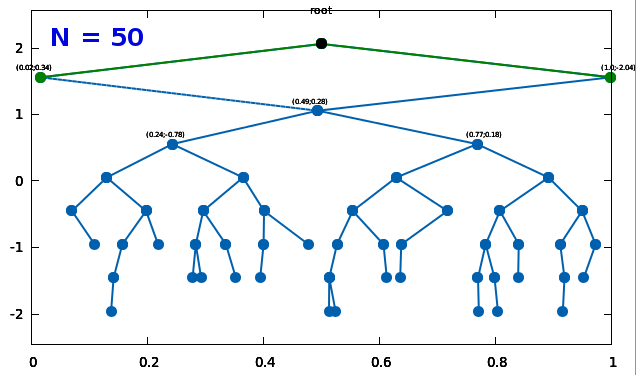
\includegraphics[scale=0.5]{tree_50}
                            \end{figure}
                        }
                        \only<4>{
                            \begin{figure}[H]
                                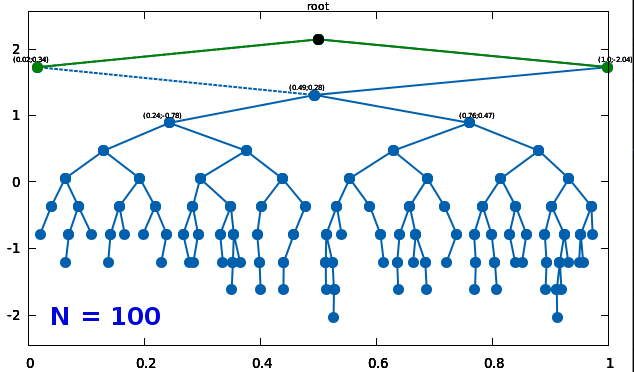
\includegraphics[scale=0.5]{tree_100}
                            \end{figure}
                        }
                    \end{frame}

                    \begin{frame}{Second step : Subsystem selection}

                        \stitle{Problems entailed by allocation $\A$ :}
                        \footnotesize
                        \begin{itemize}
                            \item<1-> \alert{Some points are badly located} : too far from their wavelet centers.
                            \item<2-> Linear system generated with previous allocation scheme \alert{may not be invertible}.
                            \item<3-> Need to \alert{extract the largest subtree $\A_S$} $\subset \A$ such that we can compute the coefficients $c_{ij}\ \forall (i,j) \in \J_S$.
                        \end{itemize}

                        \uncover<4->{
                            $\Rightarrow$ Just apply a geometric criterion to delete bad samples.
                        }

                        \uncover<5>{
                            \begin{block}{Exclusion criterion, placement condition}
                                Let $(P,\rho) \in \mathbb{R}_+^* \times \mathbb{R}_+^*$, $\A_S$ fulfills the exclusion criterion of parameters $(P,\rho)$

                                \vskip 0.2cm
                                $
                                (j,k) = \A_S(x) \in \J_{\A_S}
                                \Rightarrow 
                                \vskip 0.2cm
                                \left\{
                                    \begin{array}{l}
                                x \in\ ]\nu_{jk} - 2^{-j}\rho, \nu_{jk} + 2^{-j}\rho] \\
                        (j',k') = \A_S(x') \in \J_{\A_S}\ \mathrm{ with }\ j'<j \Rightarrow x' \not\in\ ]\nu_{jk} - 2^{-j}P, \nu_{jk} + 2^{-j}P] \\
                    \end{array}
                    \right.
                    $

                    \vskip 0.2cm
                    With \alert{$\Omega = [0,1]$} the system if invertible is $A_S$ satisfies a \alert{$(\frac{1}{2},\frac{1}{2}$)-placement condition}.
                \end{block}
            }
        \end{frame}

        \begin{frame}{Example of subtree extraction}
            \only<1>{
                \begin{figure}[H]
                    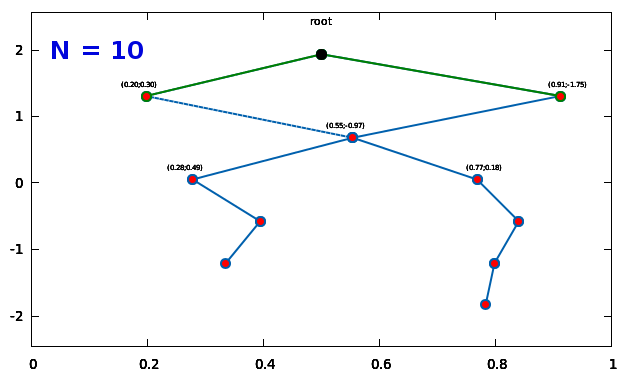
\includegraphics[scale=0.5]{tree_valid_10}
                \end{figure}
            }
            \only<2>{
                \begin{figure}[H]
                    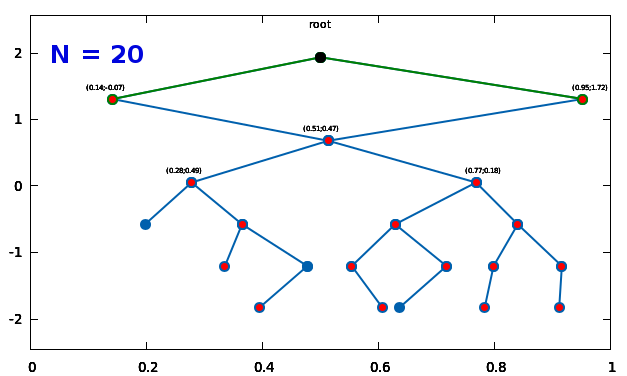
\includegraphics[scale=0.5]{tree_valid_20}
                \end{figure}
            }
            \only<3>{
                \begin{figure}[H]
                    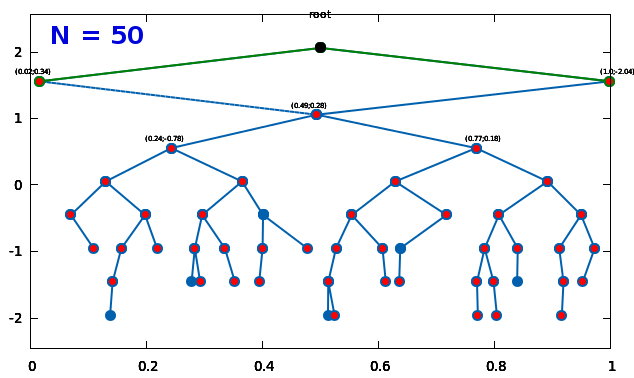
\includegraphics[scale=0.5]{tree_valid_50}
                \end{figure}
            }
            \only<4>{
                \begin{figure}[H]
                    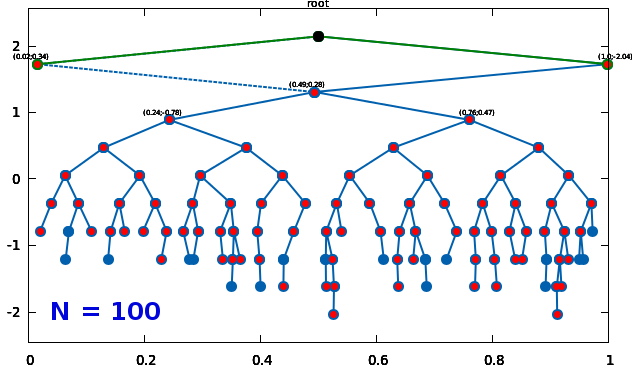
\includegraphics[scale=0.5]{tree_valid_100}
                \end{figure}
            }
        \end{frame}

        \begin{frame}{Last step : System solving}
            \stitle{Finding the coefficients $c_{ij}$ :}
            \begin{itemize}
                \item<1-> Once bad points have been removed we obtain a \stress{smaller system}.
                \item<2-> \alert{Solve square linear system of size $N_S$:}
                    \uncover<2->{
                        $$
                        \displaystyle \sum_{(j,k) \in \J_S} c_{jk} \Psi_{jk}(x) = f(x)\ \forall x \in \X_S
                        $$
                    }

                    \uncover<3->{
                        $$
                        \Leftrightarrow 
                        \left\{
                            \begin{array}{l}
                                x_i = \A_S^{-1}(j_i,k_i)\ \forall\ i \in \llbracket 0, N_S-1 \rrbracket \\
                                \displaystyle \sum_{i = 0}^{N_S - 1} c_{j_i k_i} \Psi_{j_i,k_i}(x_i) = f(x_i)\ \ \forall i\ \textrm{in}\ \llbracket 0, N_S - 1 \rrbracket
                            \end{array}
                            \right.
                            $$
                        }

                \end{itemize}
            \end{frame}

            \begin{frame}{Example of MRI at order $p = 10$}

                \titleframe{Results}

                \only<2>{
                    \begin{figure}[H]
                        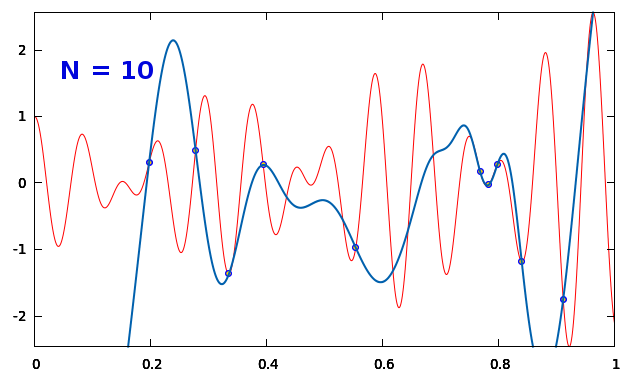
\includegraphics[scale=0.5]{fr_10}
                    \end{figure}
                }
                \only<3>{
                    \begin{figure}[H]
                        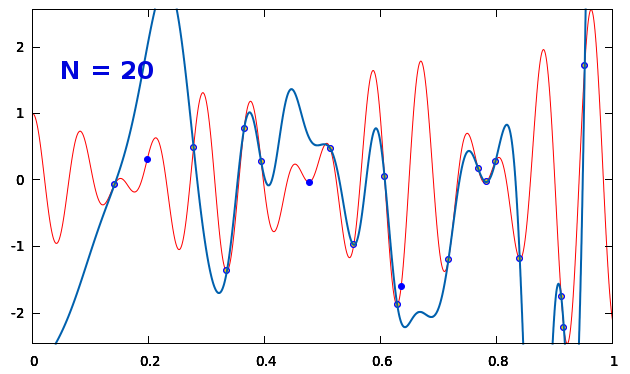
\includegraphics[scale=0.5]{fr_20}
                    \end{figure}
                }
                \only<4>{
                    \begin{figure}[H]
                        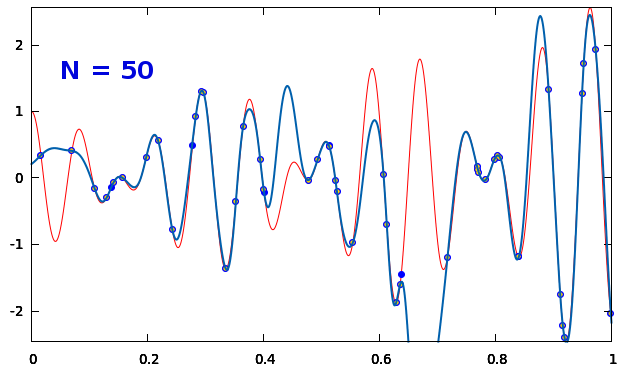
\includegraphics[scale=0.5]{fr_50}
                    \end{figure}
                }
                \only<5>{
                    \begin{figure}[H]
                        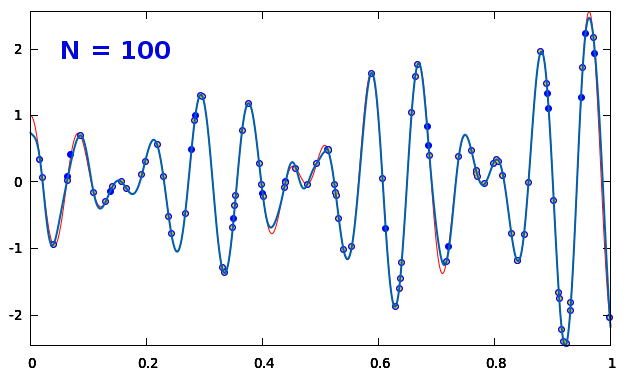
\includegraphics[scale=0.5]{fr_100}
                    \end{figure}
                }
            \end{frame}

            \begin{frame}{Error and perfomance versus order and number of samples}
                \only<1>{
                    \begin{figure}[H]
                        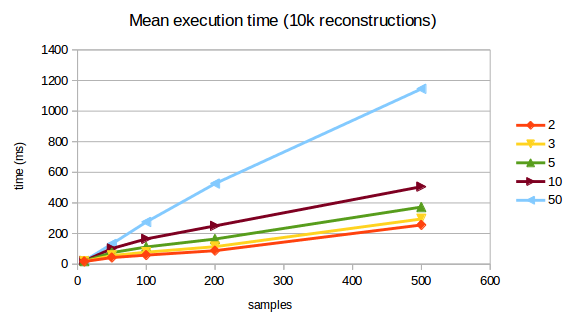
\includegraphics[scale=0.5]{execution_times}
                    \end{figure}
                }
                \only<2>{
                    \begin{figure}[H]
                        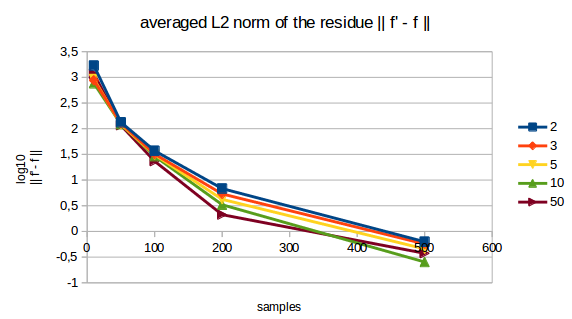
\includegraphics[scale=0.5]{residue_L2}
                    \end{figure}
                }
                \only<3>{
                    \begin{figure}[H]
                        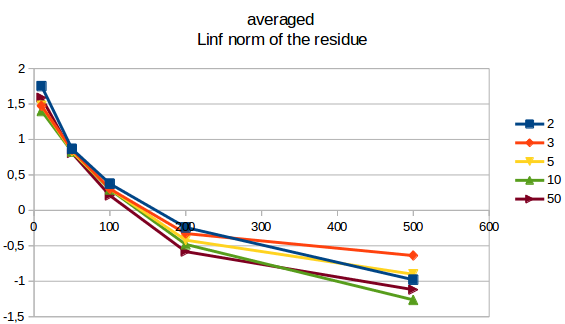
\includegraphics[scale=0.5]{residue_Linf}
                    \end{figure}
                }
            \end{frame}

            \begin{frame}{Conclusion and extensions}
                \setbeamercovered{invisible}
                \begin{itemize}
                    \item<1-> New multiresolution framework for scattered data interpolation.
                        \vspace{0.3cm}
                    \item<2-> Can be extended to more dimensions.
                        \only<1,2>{
                            \begin{figure}[H]
                                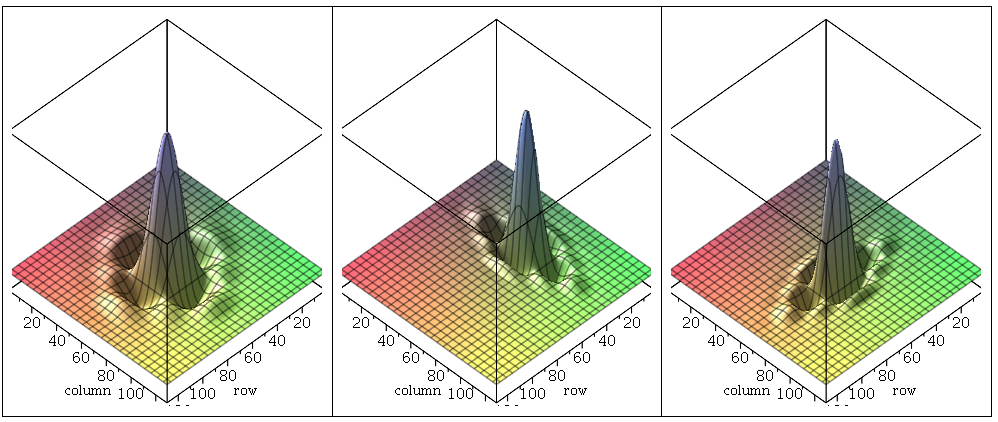
\includegraphics[scale=0.3]{3d_wavelets}
                            \end{figure}
                        }
                        \only<3->{
                            \vspace{0.3cm}
                        \item<3-> Can be adapted to any existing interpolating functions.
                            \vspace{0.3cm}
                        \item<4-> Incremental framework proposed, no need to solve the whole linear system at each sample added.
                        }
                \end{itemize}
                \vfill
            \end{frame}

            \begin{frame}{References}
                \small
                \raggedright
                \nocite{*}
                \bibliographystyle{plain}
                \bibliography{master}
                \vfill
                \begin{center}
                    \Large
                    \textcolor{titlecolor}{\textbf{Any questions ?}}
                \end{center} 
            \end{frame}

            \end{document}
